\chapter{Revisão da literatura}
\label{cap:exemplos}

% figuras estão no subdiretório "figuras/" dentro deste capítulo
\graphicspath{{\currfiledir/figuras/}}

%=====================================================

\section{A microrrede no Departamento de Engenharia Elétrica}

   O projeto da microrrede como um todo foi planejado para ser flexível com relação aos modos de operação, sendo possível utilizar conectado à rede de distribuição, quanto de forma isolada. Isso faz com que o fluxo de energia seja permitido nos dois sentidos. 

   \begin{figure}[!htb]
      \centering
      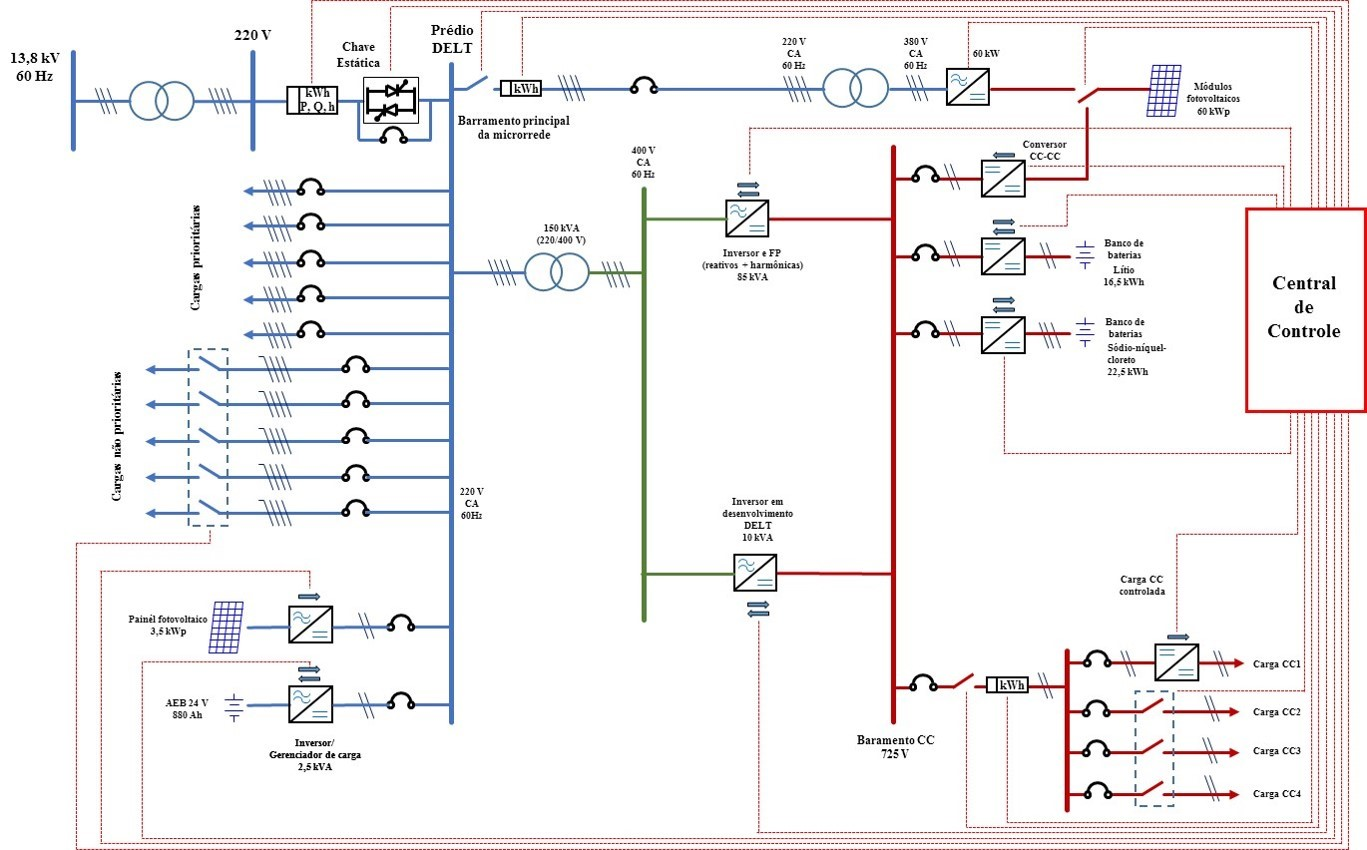
\includegraphics[width=\linewidth]{diagrama-microrrede.jpg}
      \caption{Diagrama completo da microrrede \cite{Dem19}.}
      \label{fig:diagrama-microrrede}
   \end{figure}

   A microrrede está localizada no laboratório de Eficiência Energética do Departamento de Engenharia Elétrica (DELT), no Centro Politécnico da UFPR. No diagrama da figura \ref{fig:diagrama-microrrede} podemos identificar os principais itens. Na subestação principal do compus se conecta um transformador de 350 kVA, na qual se ligam o prédio do departamento e outros prédios próximos com a tensão de 220 V. Após isso está o quadro de distribuição de energia geral. Continuando, temos uma chave eletrônica, responsável por fazer a desconexão da microrrede. 

   Parte da microrrede já está montada e é formada por um sistema de geração solar fotovoltaica de 3,5 kWp e um sistema de armazenamento de baterias de chumbo-ácido de capacidade total de 880 Ah em 24 V. Neste banco de armazenamento há um inversor e gerenciador de carga de 2,5 kW com capacidade de gerar um barramento estável monofásico em 127 V. Outros dispositivos instalados são as cargas formadas por diversos motores de indução acionando bombas d'agua, uma bomba de calor de 3 kW e um banco trifásico de capacitores com 10 kVAr.

   Está previsto ainda a instalação de três inversores, estes farão a conversão a energia proveniente de 208 módulos fotovoltaicos com um total de 65,5 kWp. Dois sistemas de armazenamento de energia serão utilizados no barramento CC de 725 V. Um será com baterias de sais de sódio-níquel-cloreto com capacidade de 22,5 kWh e os outro será com baterias de íons de lítio desenvolvidos nesse trabalho.

   Por último, ainda no barramento CC, serão conectadas várias cargas de corrente contínua, um conversor CC-CC de 30 kW e um conversor CC-CA de 85 kW. Este último é responsável pela conexão do barramento CC de 725 V em um barramento CA de 400 V. Um transformador de 150 kVA 220/400 V fará o acoplamento dos barramentos CA.

%=====================================================

\section{O carro elétrico da UFPR Formula 2020}

   Neste ano de 2020 o projeto do carro elétrico da equipe UFPR Formula está em sua terceira revisão. Nos últimos 2 anos foram usados dois motores a indução da fabricante brasileira WEG, assim como 2 inversores também da mesma fabricante. Estes tinham uma potência máxima de 20kW e nominal de 6kW cada. O sistema de armazenamento de energia utilizado em 2018 tinha 4,3 kWh, já em 2019 esse foi reduzido por vários aspectos de projeto, chegando a 3,4 kWh. Este conjunto garantia uma autonomia de cerca de 7 km.

   No projeto atual, o objetivo é se alcançar uma melhora de desempenho a ponto de competir no topo da competição nacional. Todo o projeto mecânico foi repensado pensando numa diminuição do peso e melhora da dinâmica do veículo. Já na parte elétrica, o sistema de tração foi inteiro renovado. O motor utilizado é um motor síncrono de fluxo axial da fabricante Emrax, com peso e tamanho reduzido, além de uma potência máxima de mais de 100 kW e nominal de 60 kW (a potência máxima na competição é limitada em 80 kW). O inversor é formado por um módulo de potência e um módulo de controle desenvolvido também no DELT por membros da equipe UFPR Formula. 

   Para se adequar ao novo projeto, a bateria foi inteira repensada e reprojetada. Uma nova tecnologia com maior densidade de potência e energia em relação à anterior foi escolhida, o nível de tensão foi aumentado para reduzir tamanho de componentes condutores e a capacidade foi drasticamente aumentada, para que fosse possível uma autonomia de pouco mais que 20 km (prova mais longa da competição).

%=====================================================

\section{Dispositivos fotovoltaicos}

   No uso de células fotovoltaicas, determinar o ponto de operação de máxima potência (\textit{Maximum Power Point – MPP}) é essencial para que toda a energia disponível seja utilizada \cite{Dem03}. A curva característica $I \times V$ de uma célula hipotética é apresentada a seguir (figura \ref{fig:curva-carac-fotovoltaica}), considerando a temperatura constante e em duas situações de insolação diferentes. Para que a máxima potência do módulo seja utilizada, ela deve operar nos pontos marcados como mpp. Pode-se observar que a localização do ponto no gráfico muda de acordo com a insolação, fazendo com que o controle da operação das células não seja trivial. Este controle normalmente é feito pelo dispositivo conversor acoplado às células fotovoltaicas.

   \begin{figure}[!htb]
      \centering
      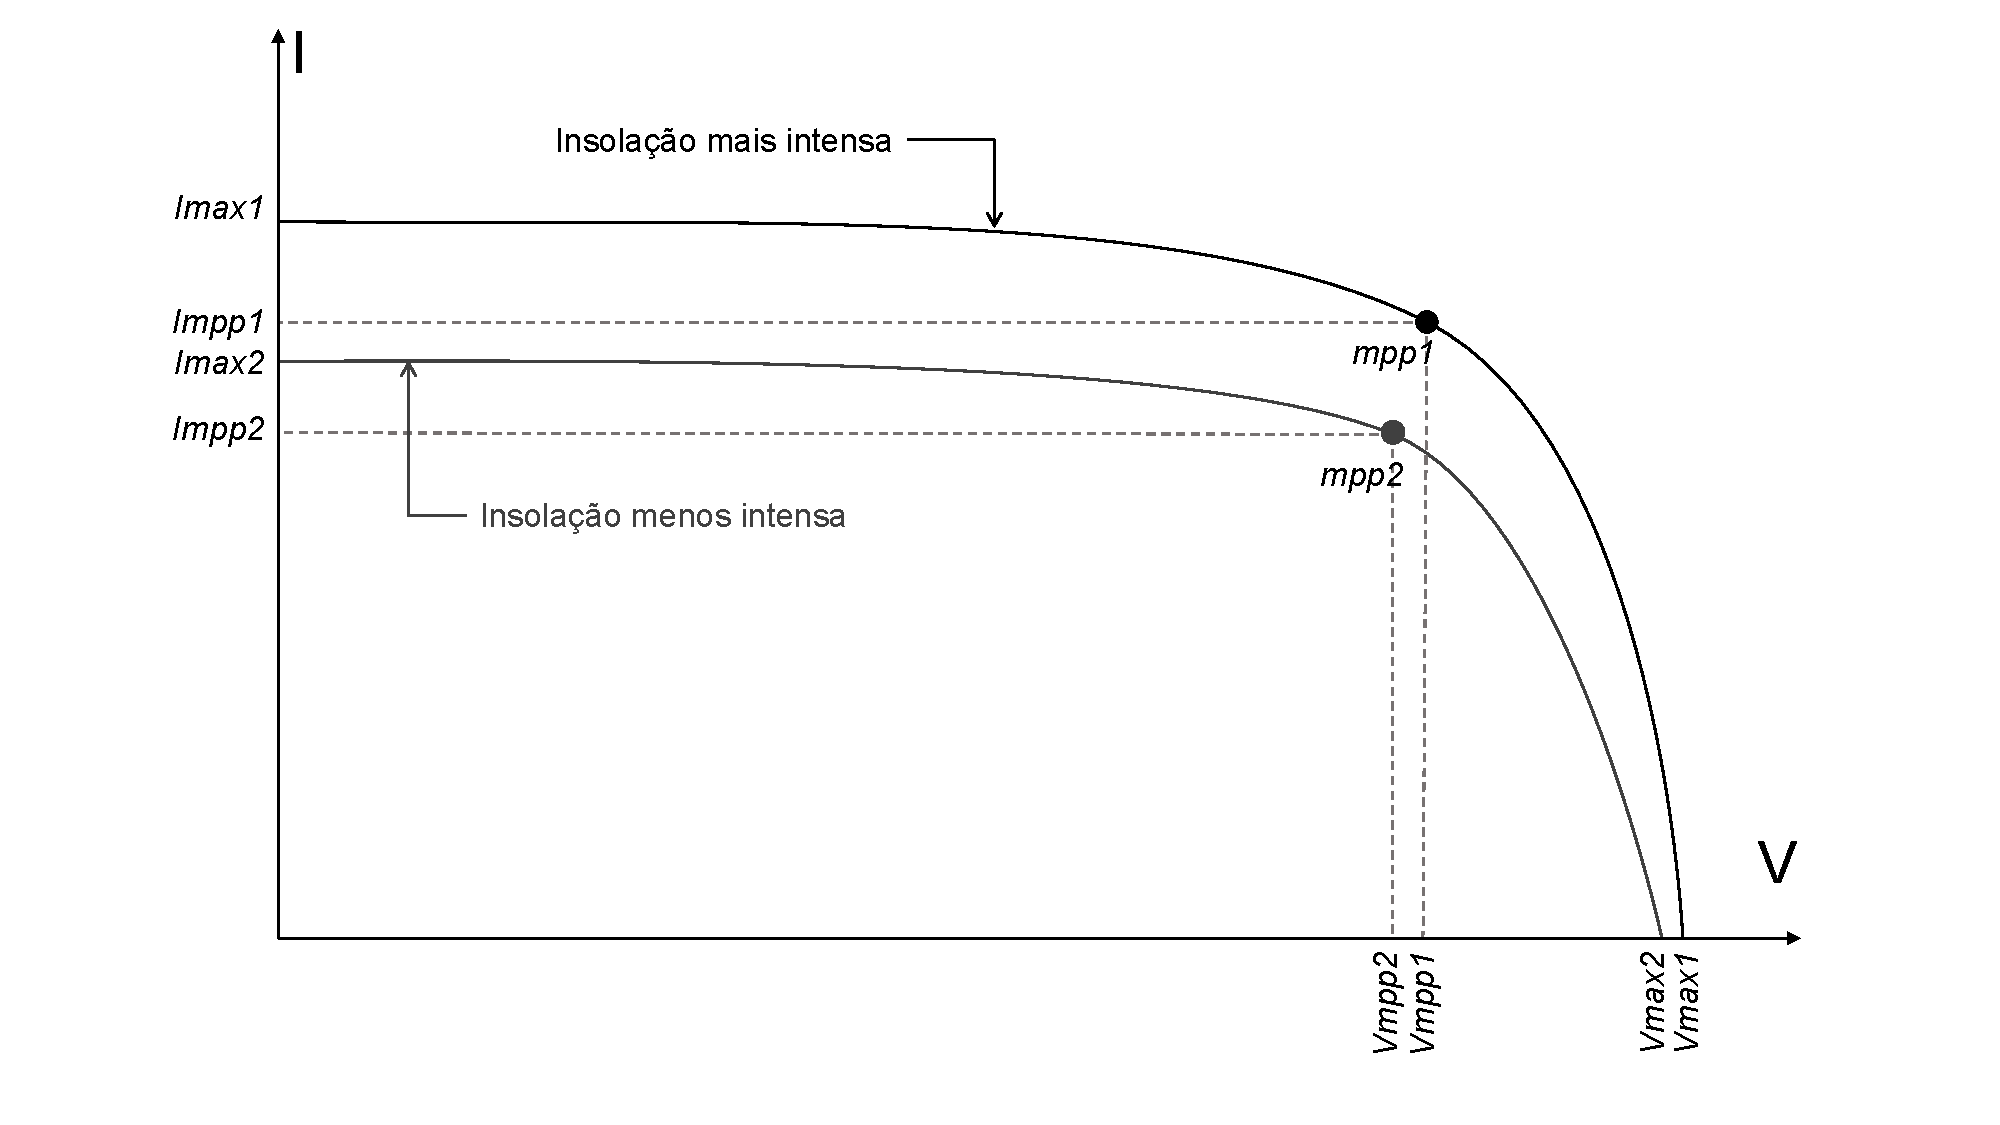
\includegraphics[width=14cm]{curva-carac-fotovoltaica.pdf}
      \caption{Curva $I \times V$ característica de célula fotovoltaica típica.}
   \label{fig:curva-carac-fotovoltaica}
   \end{figure}

   Além disso, podemos entender um dispositivo fotovoltaico pelo seu circuito equivalente, este é apresentado abaixo.

   \begin{figure}[!htb]
      \centering
      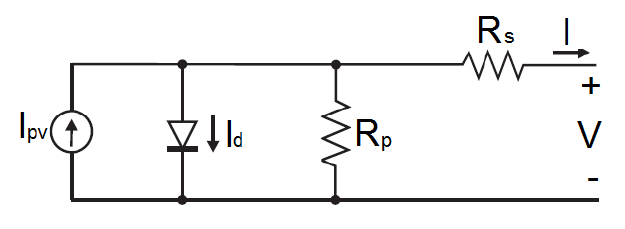
\includegraphics[height=3cm]{circ-eq-fotovoltaica.png}
      \caption{Circuito equivalente da célula fotovoltaica prática \cite{Oli16}.}
      \label{fig:circ-eq-fotovoltaica}
   \end{figure}

%=====================================================

\section{Conversores CC-CC}

   Conversores CC-CC são dispositivos formados por componentes passivos e semicondutores atuando como chave que têm por função controlar o fluxo de energia entre sua entrada e saída. Realizam isso convertendo a amplitude de tensão e corrente contínua da entrada em uma outra amplitude de saída, também em corrente contínua.

   Conversores simples têm por característica serem unidirecionais, podendo ser categorizados como abaixador, elevador ou abaixador-elevador de tensão. Considerado o conversor mais simples, o conversor abaixador de tensão, Buck, contém em sua forma mais reduzida um indutor ($L_o$), um diodo ($D$), um capacitor ($C_o$) e um semicondutor atuando como chave ($S$), como pode ser visto na figura \ref{fig:conv-buck}.

   O funcionamento exato não será discutido nesse trabalho, mas é importante saber que eles podem ser controlados pela ativação da chave $S$, alterando a frequência de ativação e outros parâmetros

   Além desses, outra categoria importante de conversor são os conversores bidirecionais, que têm por característica a habilidade de conduzir corrente nos dois sentidos, da entrada para a saída e da saída para a entrada. Uma das topologias mais simples é o conversor boost bidirecional apresentado na figura \ref{fig:conv-boost}.

   \begin{figure}[!htb]
   \centering
      \begin{subfigure}{0.48\linewidth}
         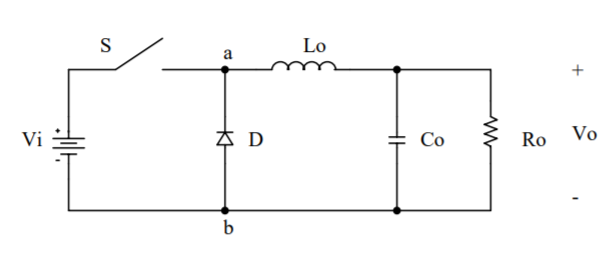
\includegraphics[height=4cm]{conv-buck.png}
         \caption{Conversor Buck \cite{Pet01}.}
         \label{fig:conv-buck}
      \end{subfigure}
      \hspace*{\fill}
      \begin{subfigure}{0.48\linewidth}
         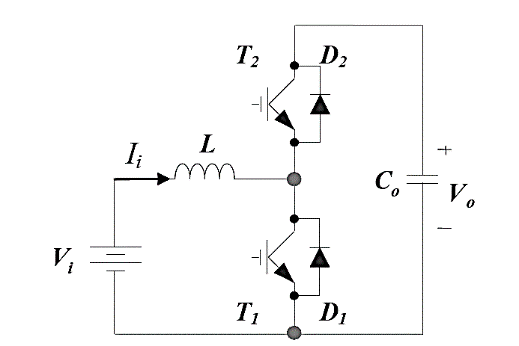
\includegraphics[height=4cm]{conv-boost.png}
         \caption{Conversor Boost \cite{Pom17}.}
         \label{fig:conv-boost}
      \end{subfigure}
   \caption{Conversores CC-CC citados.}
   \label{fig:conv-esquematicos}
   \end{figure}

%=====================================================

\section{Inversores}

   De forma semelhante aos conversores CC-CC, inversores são dispositivos formados por componentes passivos e semicondutores, mas que realizam a conversão da energia em corrente contínua para corrente alternada. É possível ainda que o sinal CA tenha uma ou mais fases, conforme necessidades do projeto. Para entendermos o funcionamento de um inversor podemos começar com o circuito mais simples: ponte H. Este é formado por apenas 4 chaves, que realizam a conexão entre a fonte e a carga (figura \ref{fig:inv-mono}). É um inversor monofásico, ou seja, gera apenas um sinal de corrente alternada de saída.

   Ele funciona invertendo a polaridade da carga conectada à fonte DC ao acionar de forma sincronizada duas chaves de cada vez, em um ciclo a chave $S1$ e $S4$, e em outro a chave $S2$ e $S3$, ou com todas as chaves abertas. Assim como os conversores CC-CC, o funcionamento não será investigado em detalhes. É importante sabermos que ele também funciona controlando a ativação das chaves com um sinal modulado na largura de pulso (PWM).

   Para que seja possível conectarmos inversores às redes de energia trifásicas ou máquinas trifásicas, precisamos também de um inversor trifásico. Este é muito semelhante à ponte H apresentada acima, mas conta com 6 chaves eletrônicas para gerar o sinal trifásico (figura \ref{fig:inv-tri}). As chaves também são acionadas de forma a gerar um sinal PWM de uma fonte senoidal, mas agora é possível que gere um sinal trifásico.

   \begin{figure}[!htb]
      \centering
         \begin{subfigure}{0.48\linewidth}
            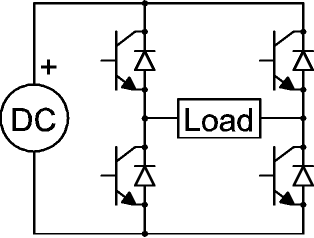
\includegraphics[height=4cm]{inv-mono.png}
            \caption{Inversor monofásico do tipo ponte H.}
            \label{fig:inv-mono}
         \end{subfigure}
         %\hspace*{\fill}
         \begin{subfigure}{0.48\linewidth}
            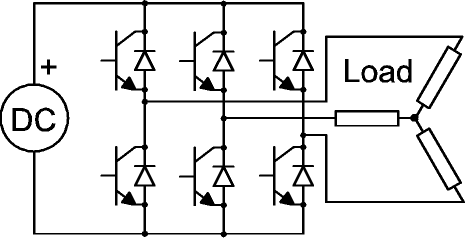
\includegraphics[height=4cm]{inv-tri.png}
            \caption{Inversor trifásico.}
            \label{fig:inv-tri}
         \end{subfigure}
      \caption{Inversores citados.}
      \label{fig:inv-esquematicos}
   \end{figure}

%=====================================================

\section{Sistemas de armazenamento de energia}

   Recentemente, a demanda de energia elétrica se tornou mais imprevisível, além disso, fontes renováveis são em sua maioria intermitentes, como a geração eólica e fotovoltaica. Sistemas de armazenamento de energia vêm para facilitar a integração dos sistemas, melhorar a estabilidade, confiabilidade, qualidade e eficiência da energia, provendo uma distribuição robusta e resiliente \cite{Zob18}.

   \subsection{Tecnologias de sistemas de armazenamento de energia}

      Várias tecnologias de armazenamento de energia vêm sendo testadas para possibilitar uma maior flexibilidade nos seus sistemas. O uso de cada uma dessas tecnologias, tem suas especificidades, variando o tempo de resposta, capacidade, dentre outros parâmetros. Na figura abaixo podemos comparar as características de potência e energia de cada tecnologia de armazenamento. Interessante é observar que baterias de íons de lítio ocupam o meio do gráfico, sendo um equilíbrio entre alta potência e energia.

      \begin{figure}[!htb]
         \centering
         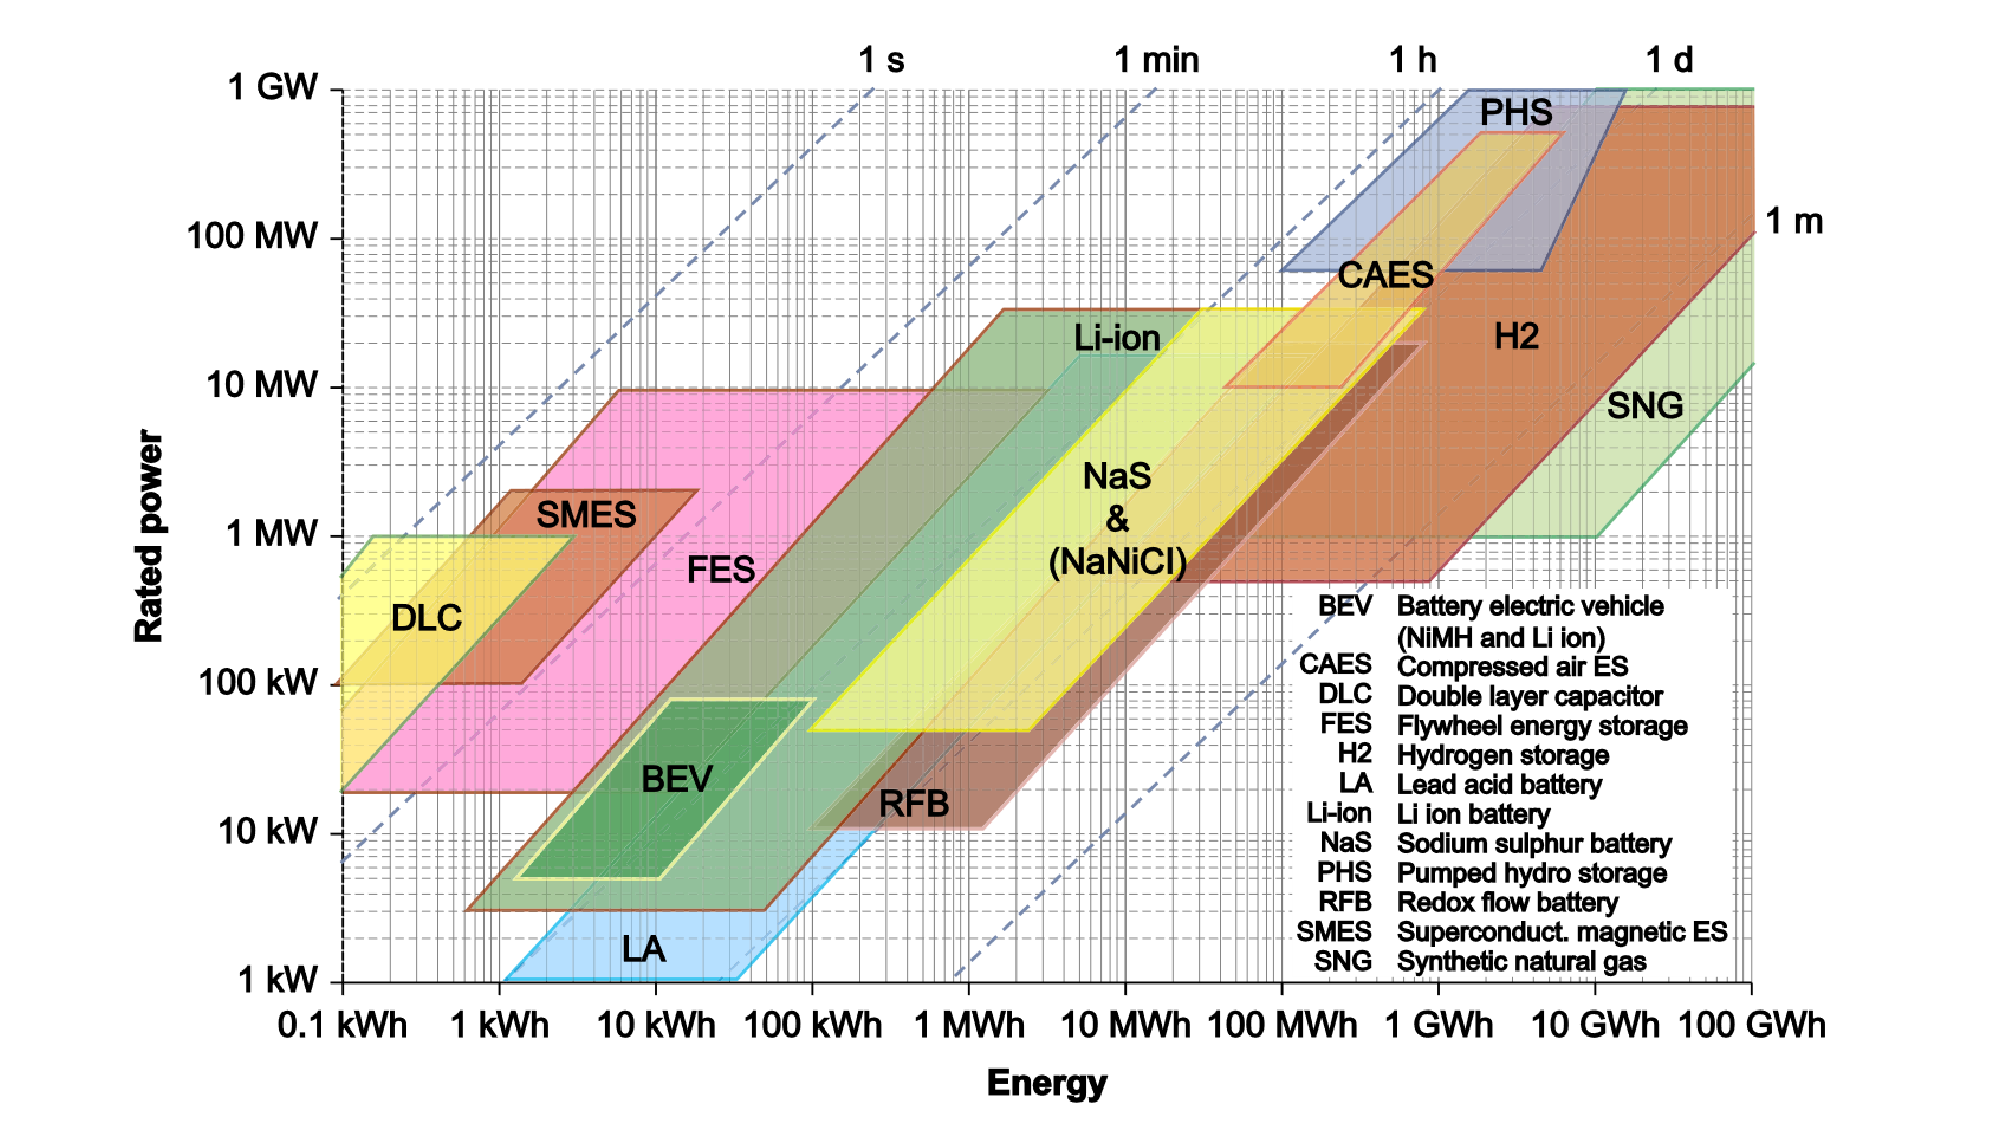
\includegraphics[width=\linewidth]{ess-ragone.pdf}
         \caption{Comparação dos parâmetros de potência e energia de diferentes sistemas de armazenamento de energia.}
         \label{fig:ess-ragone}
      \end{figure}

   \subsection{Baterias}

      Baterias normalmente são consideradas como uma invenção recente, mas foram a partir delas que surgiram os primeiros estudos no campo da eletricidade. Em 1799, Alessandro Volta (1745–1827) publicou suas descobertas ao desenvolver o que iria ser conhecido posteriormente como pilha de volta, sendo essa reconhecida como a primeira célula eletroquímica usada para o armazenamento de energia elétrica. Posteriormente, em 1859, Gaston Planté (1834–1889) desenvolve o que é considerada a primeira bateria recarregável moderna: a bateria de chumbo ácido. Esta é composta de chapas de chumbo usadas como anodo e catodo, banhadas em ácido sulfúrico, o eletrólito. Desde então, essa tecnologia vem sendo melhorada por vários pesquisadores e laboratórios ao redor do mundo, sendo hoje em dia a tecnologia com maior oferta e menor custo no mercado de armazenamento de energia em baterias \cite{War15}.

      Um outro tipo de bateria recarregável muito conhecido é a bateria de níquel cádmio (NiCd). Esta foi desenvolvida em 1899 por Ernst Waldemar Jungner (1869–1924), mas apenas por volta de 1950 se tornou comercialmente disponível. Ela se popularizou muito com o aumento do consumo de dispositivos eletrônicos portáteis, sendo a única disponível até os anos 1980. Essas baterias apresentam o efeito memória e uma menor vida útil quando comparada com outros tipos de baterias, além de serem ambientalmente danosas. Foram substituídas em sua maior parte por baterias de níquel-hidreto metálico (NiMH), que têm características muito parecidas e um impacto ambiental reduzido.

      Incentivado pelo mercado crescente de dispositivos portáteis a partir dos anos 1980, já comentado acima, inúmeras pesquisas foram desenvolvidas na tentativa de viabilizar células de íons de lítio, até então apenas teóricas. Em 1991 a Sony começa a comercialização dos primeiros dispositivos portáteis com esse tipo de tecnologia, que possui inúmeras vantagens: maior densidade de potência e energia, baixa auto descarga e não possuir o efeito memória \cite{War15}. Para resumir as características comentadas acima e trazer mais alguns detalhes, foi feita a tabela \ref{tab:bat-tecnologias} abaixo.

      \begin{table}[!htp]
         \centering
         \caption{Comparativo entre diferentes tecnologias de baterias \cite{War15}.}
         \label{tab:bat-tecnologias}
         \begin{tabular}{c m{1.9cm} m{1.9cm} m{2.2cm} m{2.2cm}}
            \hline
            \multicolumn{1}{c}{}& Chumbo ácido & Níquel cádmio & Níquel metal hidreto & Íons de lítio\footnote{Comparativo feito com bateria de íons de lítio do tipo LCO, este foi o primeiro a ser desenvolvido e comercializado.} \\
            \hline
            Descritor da química do catodo & PbA/LAB & NiCd & NiMh & LCO \\
            Energia específica (Wh/kg) & 30-40 & 40-60 & 30-80 & 120-150 \\
            Densidade de energia (Wh/L) & 60-70 & 50-150 & 140-300 & 250-450 \\
            Potência específica (W/kg) & 60-180 & 150 & 250-1000 & 600 \\
            Densidade de potência (W/L) & 100 & 210 & 400 & 1200-3000 \\
            Tensão nominal (V) & 2,0 & 1,2 & 1,2 & 3,6-3,8 \\
            Ciclos & 300-800 & 1000-2000 & 500-1500 & >700 \\
            Auto descarga (\% por mês) & 3-5 & 20 & 30 & 1-5 \\
            Temperatura de operação ($^{\circ}$C) & -20 a 60 & -40 a 60 & -20 a 60 & -20 a 60 \\
            \hline
         \end{tabular}
      \end{table}
      
   \subsection{Baterias de íons de lítio}
      \subsubsection{Funcionamento}
         Baterias são dispositivos eletroquímicos, quando olhados apenas com o olhar de engenharia elétrica é comum classificar a célula de bateria como uma caixa fechada e indivisível com propriedades normalmente apenas empíricas. Mas é importante que se tenha uma visão química por diversos motivos: a segurança do sistema é dependente da estabilidade térmica interna dos componentes das células, diferentes componentes químicos utilizados nas células podem resultar em características elétricas distintas e por consequência um circuito equivalente diferente na modelagem. 

         Na figura \ref{fig:liion-funcionamento} pode-se ver uma ilustração do funcionamento de uma célula de íons de lítio no processo de descarga. É chamado de ânodo o eletrodo com o menor potencial da reação, o polo negativo, e de cátodo o polo positivo. Em células de íons de lítio, o ânodo é de algum material carbônico e o material do cátodo varia conforme o tipo da célula. Entre os eletrodos se encontra o eletrólito e o separador: o eletrólito tem por função conduzir os componentes químicos entre os eletrodos e o separador impede que elétrons passem de um lado para o outro por dentro da célula, permitindo apenas a passagem dos íons, que são átomos de lítio com carga positiva ou negativa. Conectado nos eletrodos estão os coletores de corrente, esses têm por função conduzir os elétrons para o exterior da célula e são de material metálico.

         \begin{figure}[!htb]
            \centering
            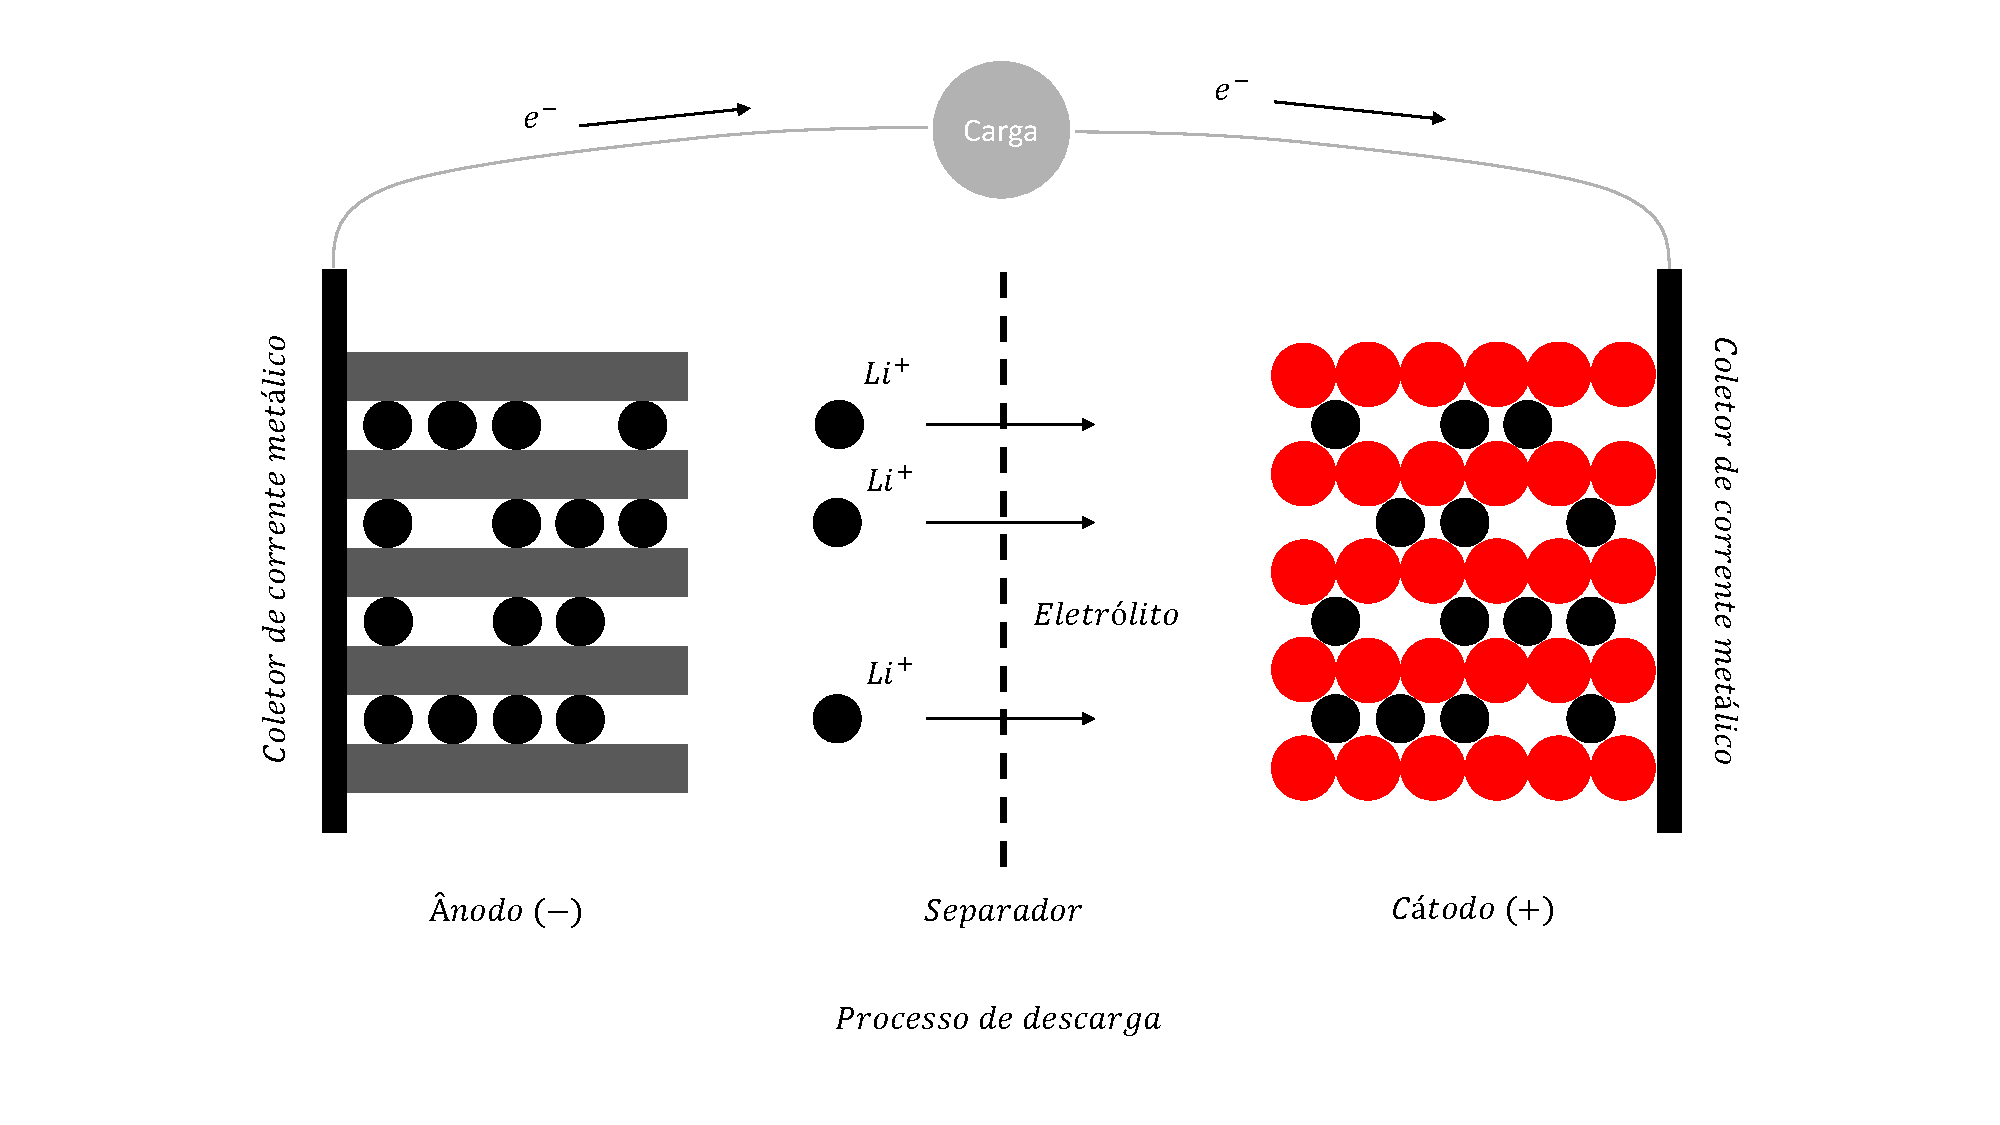
\includegraphics[width=\linewidth]{liion-funcionamento.pdf}
            \caption{Esquema de funcionamento de uma célula de íons de lítio. Adaptado de \cite{Wal18}}
            \label{fig:liion-funcionamento}
         \end{figure}
   
         A bateria ganha sua capacidade de armazenar energia elétrica quando os átomos de íons de lítio se intercalam no ânodo ou cátodo durante a descarga e a carga. Na figura \ref{fig:liion-funcionamento} está representado o processo de descarga de uma célula, sendo que na carga apenas os sentidos dos íons de lítio e da corrente se invertem.

         Baterias de íons de lítio não são apenas um tipo de bateria com uma composição química, mas sim um conjunto de diferentes tipos. Isso se dá, normalmente, pela variação dos componentes do cátodo. Tipos muito comuns são o NCA (Lítio Níquel Cobalto Alumínio) e o NMC (Lítio Níquel Manganês Cobalto) que apresentam as maiores densidades de energia. Mas é possível encontrar outros tipos com propósitos mais específicos, como LTO (Titanato de Lítio), que é muito segura e tem uma alta densidade de potência.

      \subsubsection{Formatos}
         Assim como a química varia entre diferentes células de baterias de íons de lítio, há uma variedade de formatos. Entre os principais formatos comercializados atualmente estão: células prismáticas, \textit{pouch} e cilíndricas. 

         As vantagens da célula cilíndrica incluem uma maior facilidade de fabricação e uso, resistência mecânica e um controle térmico facilitado. Um dos tamanhos mais comuns de bateria cilíndrica é o padrão 18650, medindo 18 mm de diâmetro e 65 mm de comprimento, mas variantes, como 21700 ou 20650, vêm se tornando cada vez mais comuns.

      \subsubsection{Segurança}
         Se tornou comum nos últimos anos vermos notícias de falhas em baterias de íons de lítio que causam todo tipo de problema, desde voos cancelados quando smartphones pegam fogo dentro da cabine até robô protótipo da NASA (Administração Nacional da Aeronáutica e Espaço dos Estados Unidos) sendo destruído após explosão das baterias. Assim, é necessário que tomemos todos os cuidados ao projetar um acumulador, entendendo o que leva as células à falha e prevendo formas evitar isso.

         Essa preocupação com a segurança vem de um efeito chamado \textit{Thermal Runaway} que acontece em células de íons de lítio. Que é basicamente uma reação em cadeia de aquecimento que gera um \textit{feedback} positivo até sua destruição. Em elevadas temperaturas uma decomposição exotérmica dos componentes internos da bateria começa, quando o calor gerado nessa reação é maior que a capacidade da célula de dissipar se inicia o auto aquecimento. A taxa de decomposição aumenta conforme a temperatura, seguindo a equação de Arrhenius. Eventualmente, a estabilidade da célula é perdida, o que leva à ruptura da mesma, liberando o restante da energia eletroquímica armazenada na célula. A propagação é uma reação em cadeia quando a energia liberada de uma célula se espalha para as células adjacentes, fazendo com que elas aqueçam o suficiente para iniciar a decomposição exotérmica interna \cite{Wal18}.

         \begin{figure}[!htb]
            \centering
            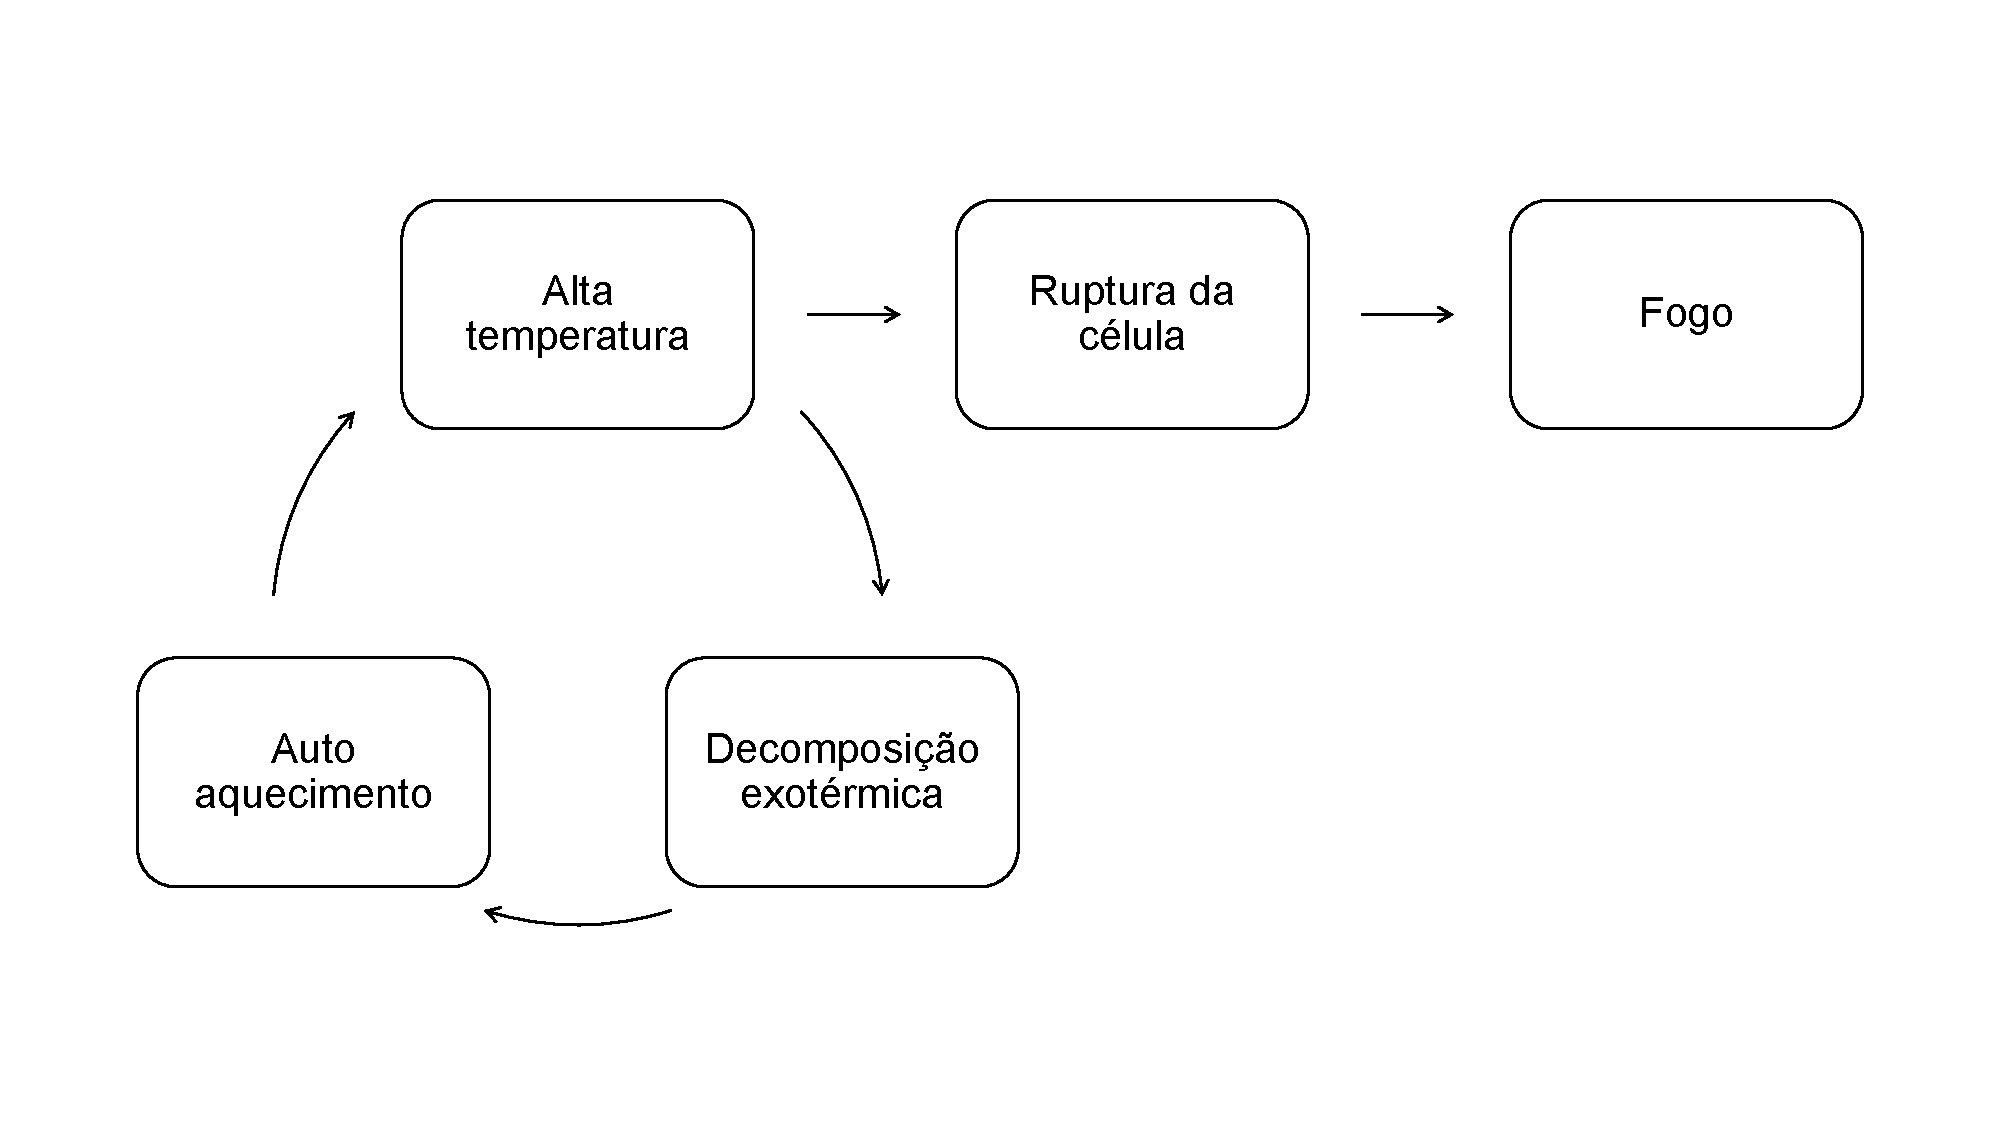
\includegraphics[width=12cm]{liion-therm-runaway.pdf}
            \caption{Esquema do funcionamento de um \textit{Thermal Runaway}}
            \label{fig:liion-therm-runaway.pdf}
         \end{figure}

         Como mostrado, essa reação se inicia com uma alta temperatura e pode ter resultados catastróficos. Mas vários motivos podem causar esse aquecimento da célula, sendo eles: a falha térmica, que seria devido à elevadas temperaturas externas; a falha mecânica, quando a célula sofre penetração ou é dobrada; curto circuito interno, normalmente causado por falhas de manufatura das células; curto circuito externo; e abuso eletroquímico, que inclui sobrecarga e sobredescarga da célula. Cada um desses motivos deve ser investigado e cuidado deve ser tomado ao projetar sistemas de mitigação de cada uma dessas falhas.

         No projeto de um acumulador é incluído um dispositivo de gerenciamento e monitoramento das células, conhecido como BMS. Esse tem por função medir a tensão, temperatura e corrente, além de ter a capacidade de controlar os dispositivos que usam a energia da bateria e em últimos casos desconectar o sistema. Um projeto mecânico sólido e bem feito do container pode prevenir falhas mecânicas, e o uso de fusíveis impedir curto-circuito.